\chapter{Introduction}
\label{chap:intro}
First of all, we encourage you to read Prof.\@ van der Aalst's guide on how to write papers~\autocite{beautiful}.

In this section, you introduce the work to your audience.
Even though this is the first chapter of your thesis, you should not necessarily write this chapter first.
It is often easier to write this chapter at the end of the thesis writing.
In this part of your introduction, i.e., the part before the Motivation section (\cref{sec:intro_ssec:motiv}), you write a paragraph (not just a sentence) for each of the bullet points mentioned in the abstract:

\begin{itemize}
	\item Domain, i.e., explain the application domain in which your thesis is applicable.
	\item Problem, i.e., motivate what the problem is you are solving.
	\item Method, i.e., describe the method you have proposed, and, compare it, briefly \& high level to other approaches. In particular, focus on the benefits of your approach versus the other approach(es)
	\item Evaluation, i.e., how did you evaluate your method and what do the results indicate?
\end{itemize}

Optionally, you can finalize this part with a little overview of what is still to come in this chapter:
\enquote{The remainder of this chapter is structured as follows.
	In \cref{sec:intro_ssec:motiv}, we motivate the need for \dots{}
	In \cref{sec:intro_ssec:probs}, we provide a formal problem statement.
	\dots
}

Before we dive into the motivation section, a few general guidelines for writing:
\begin{enumerate}
	\item Write \emph{active} and in the \emph{present tense}.
	\item Avoid \enquote{optionality} as much as possible, i.e., usage of the following words should (pun intended) be minimized:
	      \begin{itemize}
		      \item could
		      \item would
		      \item should
		      \item may
		      \item might
		      \item can
		      \item will
		      \item \dots
	      \end{itemize}
	      Good: We present a method that ...\\
	      Bad: We will present a method that ...\\
	      Good: We use function $f$ and compute its inverse.\\
	      Bad: We can use the function $f$ and will compute its inverse.
	\item Do not use \verb|\\| to generate line breaks, but an empty line % we used a few before, however do not use them in text!
	\item Position the caption of a Figure below the figure.
	\item Position the caption of a Table above the table.
	\item Write Section Headings and Titles Like This\\
	      Good: Approximation Bias in Unstable Systems\\
	      Bad: Approximation bias in unstable systems
	\item Be consistent in your references.
	      \begin{itemize}
		      \item Make sure that the name of the same author is always the same (using DBLP helps for this)
		      \item Titles should be consistent. Either use the style previously described, i.e., Approximation Bias in Unstable Systems or Approximation bias in unstable systems (this is allowed in the references, opposed to your own section headings and titles, however, \emph{BE CONSISTENT}).
	      \end{itemize}
\end{enumerate}

\section{Motivation}
\label{sec:intro_ssec:motiv}
Played-out event logs do not change, but real processes do. Following \textcite{vanderaalst2016process}, the situation in which a process is changing while being analyzed is called a concept drift. For example, two activities are concurrent at the start of an event log but then become sequential. According to \textcite{vanderaalst2016process}, typical triggers of concept drift are seasonal effects, such as higher demand in December, and changed market conditions. Classical process mining techniques mostly assume that the process at the start and at the end of the log is the same~\autocite{bose2011handling}. If a drift occurs, process models or key performance indicators (KPIs) computed over the entire log mix two different processes. The process owner must therefore detect whether and when the process changed, and what changed.

A drift does not restrict itself to the order of activities. Processes run in a context, but process analysis sometimes ignores it. As described by \textcite{vanderaalst2016process}, process context covers how cases influence each other like competing for the same resources. A single case is therefore not sufficient to explain the observed behavior alone. Thus, for successful explanation of the observed behavior and changes, dependencies inside the cases as well as between the cases and dependencies with the resources need to be analyzed. This leads to the terms of intra-case dependencies and inter-case dependencies introduced by \textcite{senderovich2017intra}. This thesis takes on the terminology and considers a process from three perspectives:
\begin{itemize}
	\item \emph{Intra-case perspective:} The history of a single case up to a specific time, covering which activities happened in which order and how often. Drift example: A new trace variant dominates.
	\item \emph{Resource perspective:} The working style of resources, such as their workload, service times, handovers, and the activities they perform. Drift example: A resource no longer exists and other resources take over the work.
	\item \emph{Inter-case perspective:} The current situation of all running cases of the process, covering arrivals, waiting times, and case attributes. Drift example: The mean waiting time between consecutive events of a case increases.
\end{itemize}

From all three perspectives concept drifts can take place, but they can also influence each other. For example, a new trace variant with a frequent activity becomes dominant (intra-case perspective). The resource responsible for that activity then has more work to do (resource perspective), which affects the waiting times in the entire process (inter-case perspective).

We describe each drift by three properties:
\begin{itemize}
	\item \emph{Drift type:} What changes, e.g., the control-flow, the reassignment of an activity to another resource, or the waiting time between consecutive events.
	\item \emph{Drift perspective:} The perspective to which the drift type belongs. For example, control-flow drifts belong to the intra-case perspective, reassignment drifts to the resource perspective, and waiting time drifts to the inter-case perspective.
	\item \emph{Drift mode:} How fast the change takes effect, i.e., suddenly or gradually.
\end{itemize}
In the literature the terms drift type, drift mode and drift perspective are used interchangably. We reserve the term drift type for what changes, the term drift mode for how it changes and the tern drift perspective in classificational manner for drift types.

Existing concept drift detection approaches cover this picture only partially:
\begin{itemize}
	\item \emph{Control-flow focus:} Most of the work on drift detection focuses on control-flow. Out of the 38 drift detection papers in the survey of \textcite{sato2022survey}, only six focus on the time perspective, three on the data perspective, and none on the resource perspective. In our framework, waiting times and case attributes fall under the inter-case perspective, and service times under the resource perspective. A concept drift that only changes the time or resource perspective stays undetected with control-flow approaches.
	\item \emph{Single KPIs:} Approaches beyond control-flow often track single KPIs. \textcite{adams2023explainable} turn each KPI chosen by the user into a time series over time windows and detect drifts in each series separately. A drift therefore shows up as separate change points in several KPIs. This approach does not deliver a compact description of the overall process situation. For steady-state detection, \textcite{kraus2026steady} show that combining complementary process characteristics is more accurate than relying on a single one.
	\item \emph{Drift modes:} How fast a change takes effect is also important information for the process owner. Most of the existing approaches focus on sudden drifts only~\autocite{sato2022survey}.
	\item \emph{Missing test data:} \textcite{sato2022survey} argue that real-world logs are unsuitable for measuring detection accuracy, since their drift points are unknown. They find only three public synthetic datasets with injected drifts. These datasets cover only the control-flow and time perspectives and do not mix different drift modes. None of them contains a resource drift or a change in case arrivals. A recent benchmark by \textcite{padella2026everything} injects drifts into five real logs, but again only into the control-flow and activity durations.
\end{itemize}

\begin{figure}[tb]
	\centering
	\definecolor{stateA}{RGB}{0,114,178}
	\definecolor{stateB}{RGB}{230,159,0}
	\definecolor{stateC}{RGB}{0,158,115}
	\definecolor{stateD}{RGB}{204,121,167}
	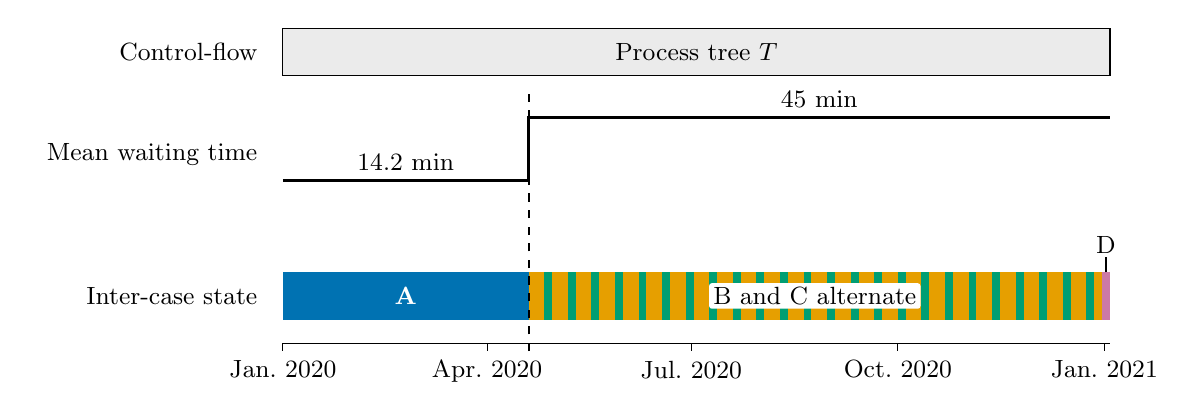
\begin{tikzpicture}[font=\small]
		% row labels
		\node[anchor=east, align=flush right, text width=2.8cm] at (3.2, 3.7) {Control-flow};
		\node[anchor=east, align=flush right, text width=2.8cm] at (3.2, 2.4) {Mean waiting time};
		\node[anchor=east, align=flush right, text width=2.8cm] at (3.2, 0.6) {Inter-case state};
		% one x unit is one day from January 1, 2020
		\begin{scope}[xshift=3.4cm, x=0.0285cm]
			% control-flow: one process tree over the whole log
			\draw[fill=black!8] (0, 3.4) rectangle (368.5, 4.0) node[midway] {Process tree $T$};
			% waiting time: 0.026 cm per minute above the baseline y = 1.7
			\draw[very thick] (0, 2.07) -- (109.5, 2.07) -- (109.5, 2.87) -- (368.5, 2.87);
			\node[above] at (54.75, 2.07) {14.2~min};
			\node[above] at (239, 2.87) {45~min};
			% inter-case states
			\fill[stateA] (0, 0.3) rectangle (109.5, 0.9);
			\node[white, font=\small\bfseries] at (54.75, 0.6) {A};
			\begin{scope}
				\clip (109.5, 0.3) rectangle (365, 0.9);
				\foreach \i in {0,...,24} {
					\fill[stateB] ({109.5 + 10.5 * \i}, 0.3) rectangle ++(7, 0.6);
					\fill[stateC] ({116.5 + 10.5 * \i}, 0.3) rectangle ++(3.5, 0.6);
				}
			\end{scope}
			\node[fill=white, inner sep=1.5pt, rounded corners=1pt] at (237, 0.6) {B and C alternate};
			\fill[stateD] (365, 0.3) rectangle (368.5, 0.9);
			\draw (366.75, 0.9) -- (366.75, 1.1) node[above, inner sep=1pt] {D};
			% time axis
			\draw (0, 0) -- (368.5, 0);
			\foreach \pos/\lab in {0/Jan.\ 2020, 91/Apr.\ 2020, 182/Jul.\ 2020, 274/Oct.\ 2020, 366/Jan.\ 2021}
				\draw (\pos, 0) -- (\pos, -0.1) node[below] {\lab};
			% drift point, below the control-flow row
			\draw[dashed, thick] (109.5, -0.1) -- (109.5, 3.2);
		\end{scope}
	\end{tikzpicture}
	\caption[Motivating example: a waiting-time drift that control-flow does not show]{%
		Visualization of the synthetic Rheon log generated with a mean waiting time drift.
		At the drift point (dashed), the mean waiting time between consecutive events of a case rises from 14.2 to 45~min, while all cases still follow process tree~$T$.
		The inter-case state of each 12-hour window switches exactly there from A to an alternation of B and C.
		State D marks the run-out of the log after the last case arrivals.
		The alternation of B and C is drawn schematically.}
	\label{fig:intro:motivation}
\end{figure}

\Cref{fig:intro:motivation} shows this gap using a synthetic event log generated by Rheon. Rheon is our generator for synthetic event logs with injected concept drifts in all three perspectives (\cref{chap:rheon}). This log has 300,299 cases with 1,946,540 events, seven activities, and seven resources. Its cases arrive between January 1 and December 31, 2020. On April 19, 2020, the mean waiting time between consecutive events of a case jumps from 14.2 minutes to 45 minutes. The activities, the control-flow, the resources, and the dominant resource of each activity remain unchanged. A detector that only compares relations between activities sees the same control-flow before and after the drift point and misses the change.

The state-based approach of this thesis aims to detect drifts in all three perspectives and to show what changed. Instead of separate change points per KPI, our states combine many features into one compact description. Rheon provides test logs with known drift points in all three perspectives. In \textcite{berti2025ocel}, execution states from object-centric event logs are computed for objects. We adapt the approach from objects to cases in our case-centric framework and define our intra-case states. As an extension to their work, our approach also takes into account resource and inter-case perspectives and adapts the idea to them.

Overall, we compute states from an event log by extracting features, compressing, and clustering. The input of our approach is an event log, and the output consists of intra-case, resource, and inter-case states whose changes over time indicate drifts. In \cref{fig:intro:motivation} one can visually see the general idea of our approach for the inter-case perspective. We describe each 12-hour window by features such as the number of active cases, arrivals, completions, and the mean waiting time between consecutive events of a case. Following the execution states of \citeauthor{berti2025ocel}, a principal component analysis (PCA) compresses these features. A $2 \times 2$ self-organizing map (SOM) is trained on these compressed feature vectors. Each of its four cells is one state, and each window gets the state of its best-matching cell.

The pipeline is unsupervised and does not see the drift point or the drift type. As seen in \cref{fig:intro:motivation}, all 219 windows before the drift point fall into state~A. From the drift point until December~31, the windows alternate between states~B and~C. The last seven windows, in which the log runs out, form state~D. The first principal component explains 51\% of the variance and is dominated by the mean waiting time between consecutive events of a case. It therefore also shows what changed: after the drift point, more time passes between the events of a case.

\section{Problem Statement}
\label{sec:intro_ssec:probs}
An event log records a process over a long period, and the process often changes within this period. Such a concept drift affects the intra-case, resource, or inter-case perspective, or several of them at once. A detector that only captures control-flow drifts therefore misses drifts that only affect the resource or inter-case perspective.

\Textcite{vanderaalst2016process} names three main challenges in dealing with concept drifts:
\begin{enumerate}
	\item\label{item:intro:change_point} \emph{Change point detection}: Did the process change? If yes, when did it change?
	\item\label{item:intro:change_localization} \emph{Change localization and characterization}: What has changed?
	\item\label{item:intro:change_process} \emph{Change process discovery}: How to capture and predict second-order dynamics?
\end{enumerate}

According to \citeauthor{vanderaalst2016process}, a process is not static even when there is no drift (first-order dynamics). This makes it even harder to detect changes of the process itself (second-order dynamics). Most approaches compare sliding windows of events with statistical methods. To localize drift points exactly and detect them at different time scales, the window length must vary. Moreover, drifts at different time scales can overlap, as in~\cref{fig:intro:drift_windows}.

This thesis focuses on challenges~\ref{item:intro:change_point} and~\ref{item:intro:change_localization}. To characterize a drift, our framework determines its drift perspective, its drift mode, and what exactly changed.

In conclusion, this thesis focuses on the following problem:
\begin{itemize}
	\item \emph{Given:} An event log in which each event belongs to exactly one case. Each event carries a case ID, an activity, and a timestamp, and optionally a resource and case attributes. Drift points, drift types, drift perspectives, and drift modes are unknown.
	\item \emph{Objective:} Compute intra-case, resource, and inter-case states whose changes over time indicate drifts. From these changes, detect the drift points and determine for each drift its perspective, its mode, and what changed.
	\item \emph{Evaluation:} We compare the detected drift points with known drift points in two sets of logs. First, synthetic Rheon logs contain drifts in all three perspectives. Second, the benchmark of \textcite{padella2026everything} injects sudden, gradual, and recurring control-flow and duration drifts into five real logs.
\end{itemize}

\begin{figure}[tb]
	\centering
	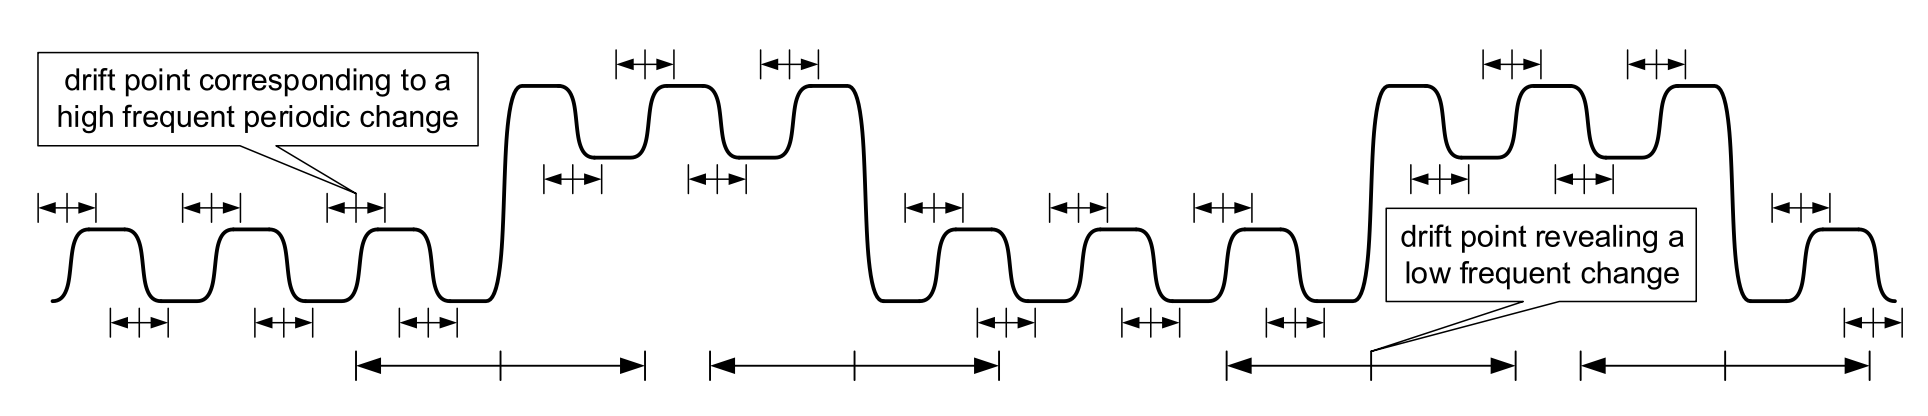
\includegraphics[width=\textwidth]{figures/vanderaalst_drift_sliding_windows}
	\caption[Drifts on two different time scales]{
		A periodically changing process with drifts at two different time scales, taken from \textcite{vanderaalst2016process}. Shorter sliding windows are used to detect short-term drifts. The left half of each sliding window is compared with the right half to spot statistically relevant changes. The larger sliding windows at the bottom are used for long-term drifts.}
	\label{fig:intro:drift_windows}
\end{figure}

\section{Research Questions}




\section{Research Goals}

In this section, you present your research goals.
A research goal is a concise statement that s.t., achieving the goal helps you in (partially) solve a research question.
Hence, the research questions and goals are often very related.
Furthermore, it should be obvious for the reader what goal answers what problem.

In the context of our previously mentioned questions, some example goals are:
\begin{itemize}
	\item Conduct a systematic literature review on noise patterns in real event data.
	\item Design a noise detection algorithm.
	\item Formalize the notion of incompleteness in an event log.
	\item \dots
\end{itemize}

\section{Contributions}

In this section, you list the contributions that your thesis makes to our wonderful world (of science).
Again, there is a strong link to the previous section.
Usually, you have achieved your research goals.
Hence, the contributions are concrete statements of the goals you have achieved.
Additionally, your evaluation (most likely also stressed as a goal) is a contribution.
Any implementation or prototype can also be quantified as a contribution.

Some examples:
\begin{itemize}
	\item A systematic literature review covering 35 articles on noise patterns in real event data
	\item A noise detection algorithm based on dynamic programming and symbolic linking
	\item ...
\end{itemize}

\section{Thesis Structure}
In this section, you outline the remainder of the thesis.

The remainder of this thesis is structured as follows.
In \cref{chap:related_work}, we discuss related work.
In \cref{chap:prelim}, we present basic mathematical preliminaries, used throughout the thesis.
